\part{Novell Open Enterprise Server 2}
Novell OES2 представляет собой законченное решение по предоставлению базовых сетевых сервисов - регистрация пользователей в сети, сетевая печать, порталы доступа и управления. OES2 может заменить собой любую из существующих систем на базе Linux/Netware/Windows, а присутствующий инструменты миграции обеспечат плавную миграцию данных. Решение построено на базе открытой платформы SUSE Linux Enterprise Server 10 (SLES10) с добавлением функционала коммерческих сервисов Novell. Весомым преимуществом решения можно назвать его высокую степень интегрированности и веб-ориентированности. Управления сетью OES2 сильно проще и удобнее чем даже Windows, а гибкость настройки не ниже чем у любой Linux-системы.

\section{Получение дистрибутива}
Как уже говорилось, решение построено на базе SLES10. Соответственно для установки нам в первую очередь потребуется этот дистрибутив. Дополнительные сервисы вынесены в отдельный диск, функционально являющийся Add-on для SLES10.\par
Чтобы скачать все необходимые пакеты необходимо зарегистрироваться на портале www.novell.com (регистрация бесплатна).\par
Последнюю версию OES2 можно найти на странице novell.com\footnote{http://www.novell.com/products/openenterpriseserver/}. Для установки потребуется скачать SLES10 (32 или 64-битную платформу). Плюс к этому скачиваем диск начинающийся на OES2 (соответственно выбранной платформе).
\clearpage

\section{Установка}
Начало установки.\par
Установка начинается с загрузки сервера с диска SLES10 DVD1. Диск с сервисами OES2 пригодится несколько позже, во время настройки. Если загрузка удалась, то вы увидите следующее окно.
\begin{figure}[H]
\center{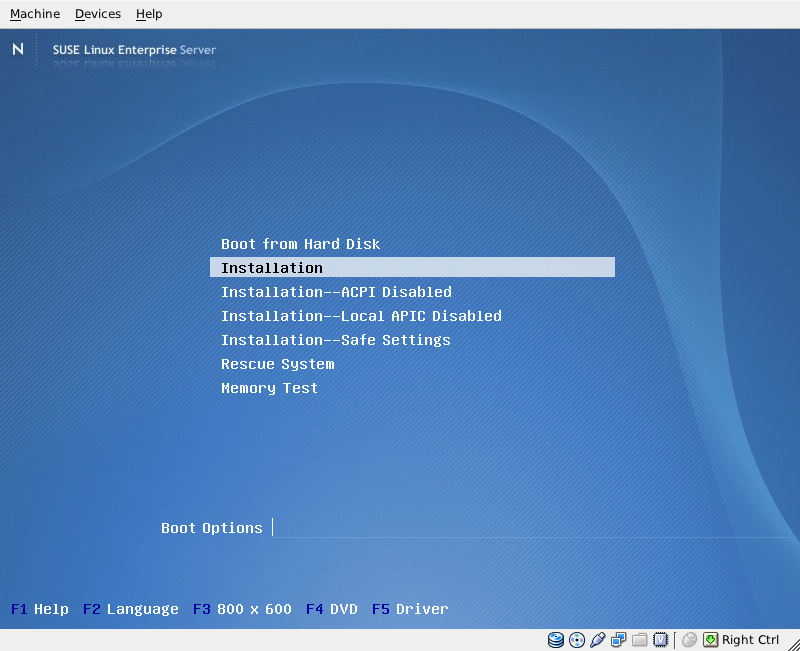
\includegraphics[width=1\linewidth]{oes/1.png}}
\caption{Начало установки}
\label{fig1}
\end{figure}
По умолчанию выбран пункт <<Boot from Hard Disk>> (Загрузка с жёсткого диска). Для начала установки выбираем пункт <<Installation>>.
\clearpage

Первое окно — выбор языка установки, выбираем <<Русский>>, нажимаем <<Применить>>.
\begin{figure}[H]
\center{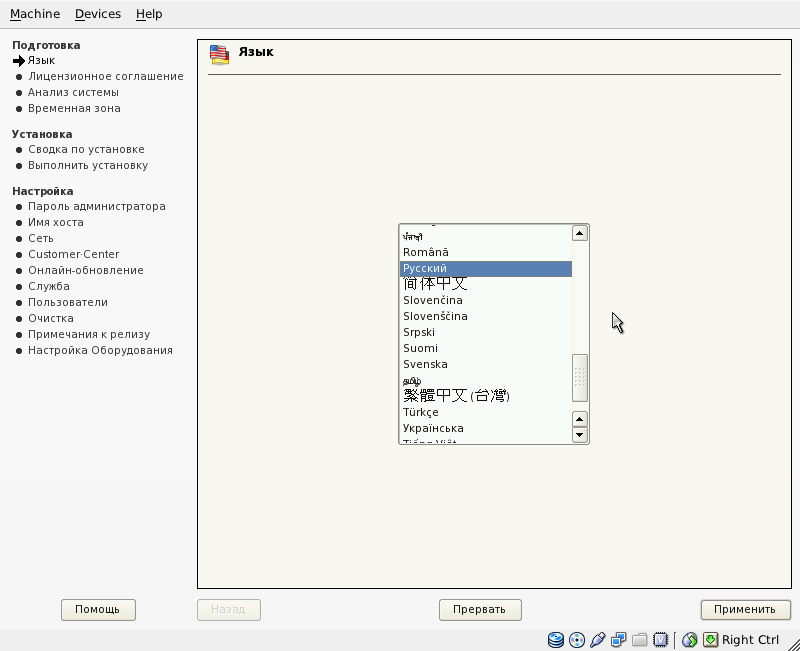
\includegraphics[width=1\linewidth]{oes/2.png}}
\caption{Выбор языка}
\label{fig2}
\end{figure}
\clearpage

Далее предлагается принять лицензию на SLES10 <<Да, я согласен с условиями лицензионного соглашения>>, без чего дальнейшая установка невозможна.
\begin{figure}[H]
\center{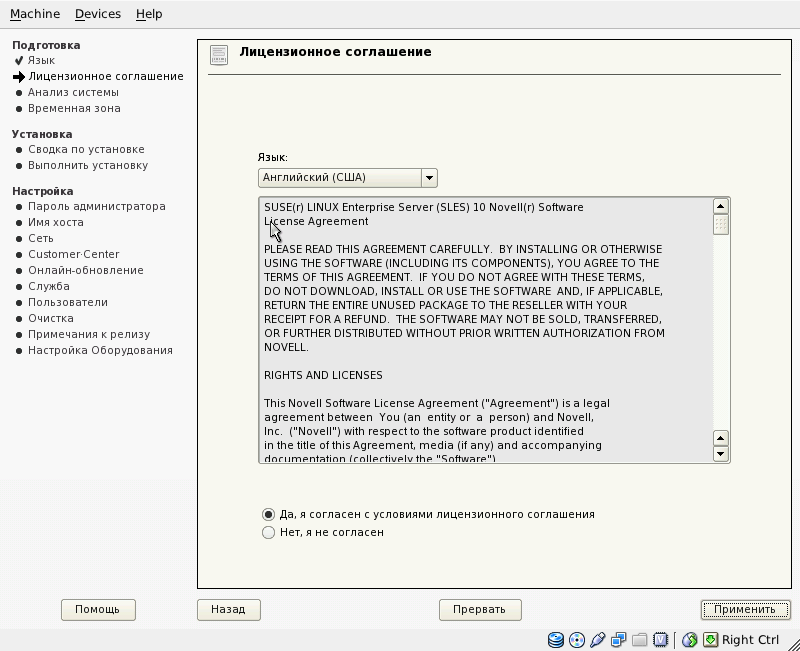
\includegraphics[width=1\linewidth]{oes/3.png}}
\caption{Лицензионное соглашение}
\label{fig3}
\end{figure}
\clearpage

Установщик автоматически предлагает вариант <<Новая установка>>. Если бы на сервере была установлена какой-либо SUSE Linux, то был бы доступен выбор варианта обновления.
\begin{figure}[H]
\center{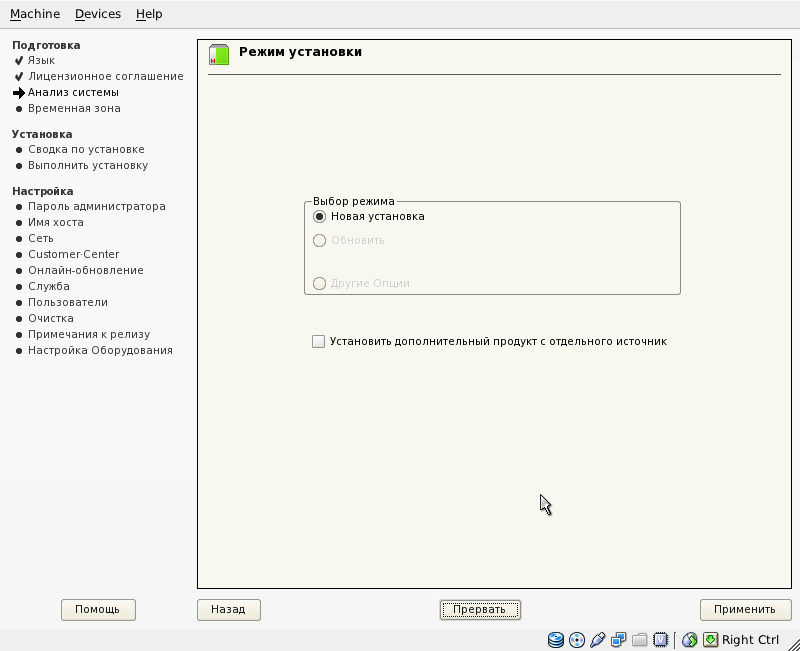
\includegraphics[width=1\linewidth]{oes/4.png}}
\caption{Выбор режима установки}
\label{fig4}
\end{figure}
\clearpage

После выбора временной зоны появляется итоговая сводка. Это последний этап конфигурирования системы перед установкой. На последующих шагах для настройки NSS\footnote{Novell Storage Services (NSS) - файловая система, используемая в Novell для создания томов на файловом сервере} нам потребуется свободное дисковое пространство. Для этого можно выделить отдельный жесткий диск (или же поднять для этих целей отдельностоящий сервер). В нашем случае мы переразобъём текущий раздел, выделив свободное место на нём.
\begin{figure}[H]
\center{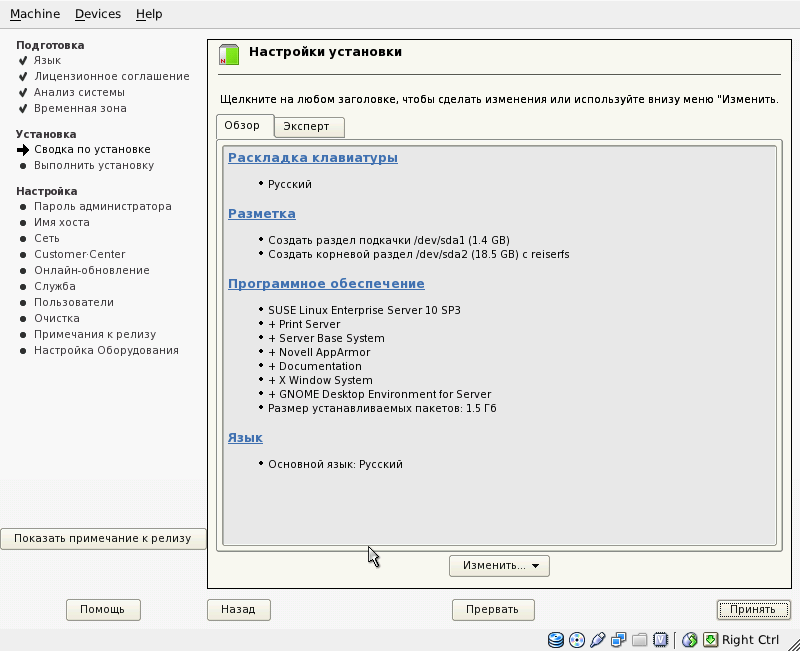
\includegraphics[width=1\linewidth]{oes/p1.png}}
\caption{Сводка установки}
\label{p1}
\end{figure}
Заходим в раздел <<Разметка>>.
\clearpage

Полностью переделывать разметку мы не будем, поэтому выбираем пункт <<Настроить раздел согласно предложению>>.
\begin{figure}[H]
\center{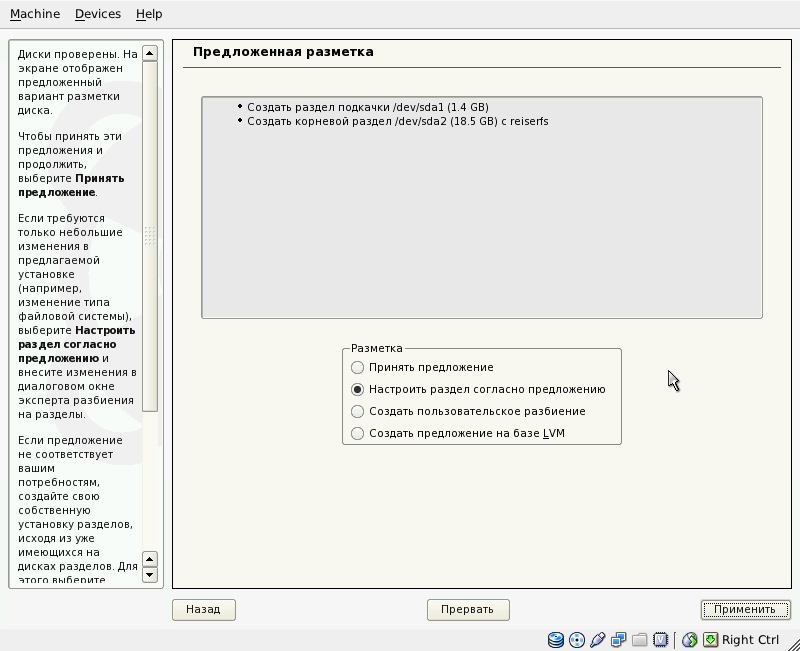
\includegraphics[width=1\linewidth]{oes/p2.png}}
\caption{Предложенная разметка}
\label{p2}
\end{figure}
\clearpage

Здесь мы уменьшим основной раздел нажав кнопку <<Изменить размер>>.
\begin{figure}[H]
\center{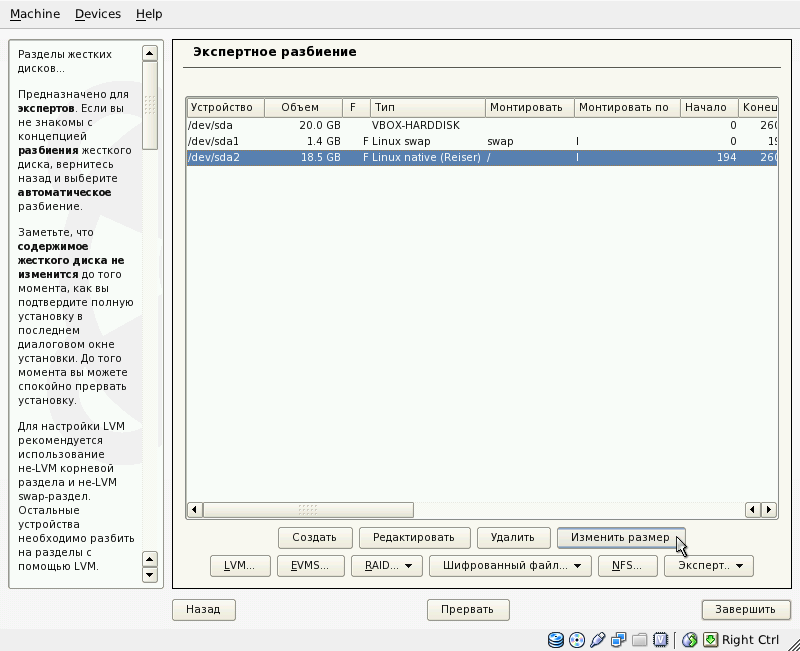
\includegraphics[width=1\linewidth]{oes/p3.png}}
\caption{Изменение разметки}
\label{p3}
\end{figure}
\clearpage

Отрезаем часть от раздела. В будущем мы используем это свободное пространство для создания NSS томов.
\begin{figure}[H]
\center{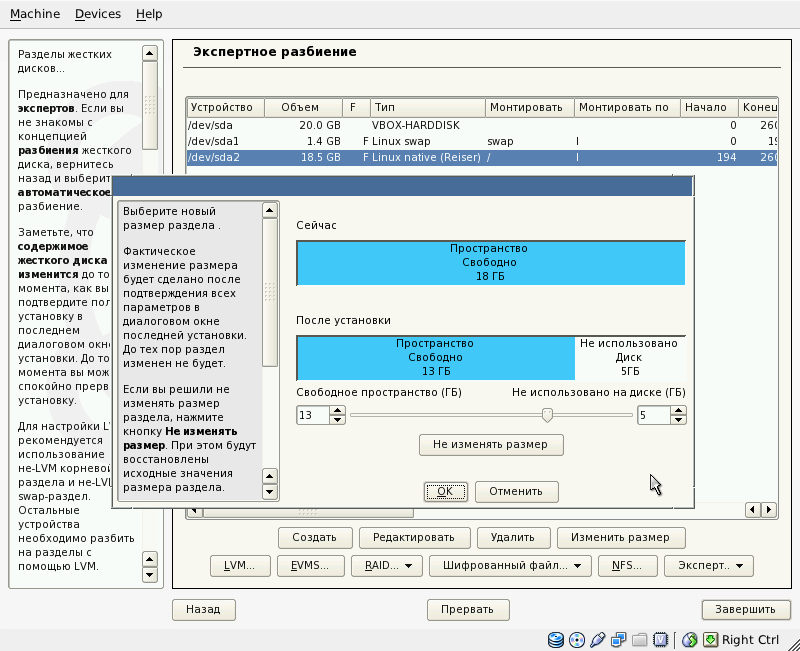
\includegraphics[width=1\linewidth]{oes/p4.png}}
\caption{Изменение разметки}
\label{p4}
\end{figure}
\clearpage

Теперь у нас появилось немного свободного дискового пространства, можно приступать к установке, нажав <<Принять>>.
\begin{figure}[H]
\center{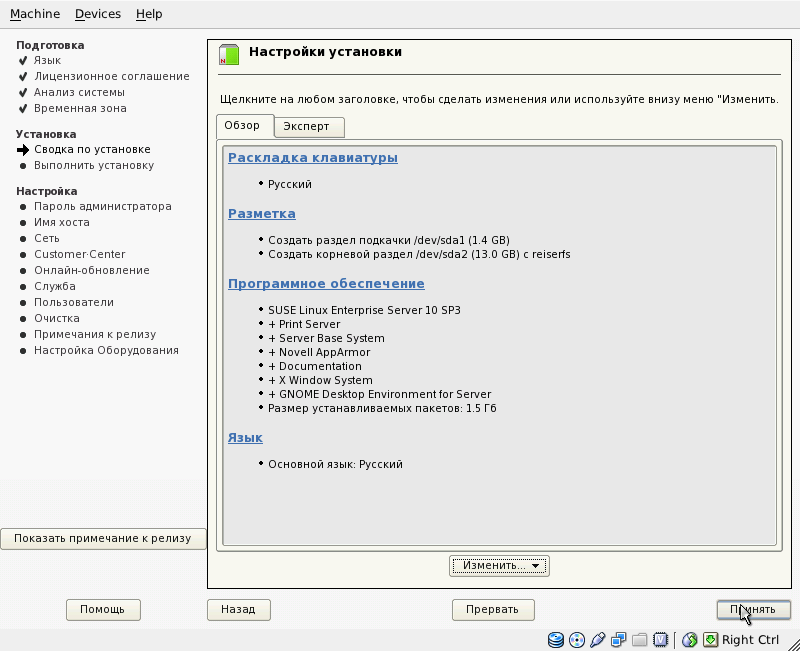
\includegraphics[width=1\linewidth]{oes/p5.png}}
\caption{Сводка установки}
\label{p5}
\end{figure}
\clearpage

После перезагрузки мы можем приступить к первоначальной настройке сервера.\\
Начинаем с пароля администратора root. Если пароль указать недостаточно стойким или присутствующим в базе типовых паролей, то система выдаст предупреждение о потенциальной угрозе.
\begin{figure}[H]
\center{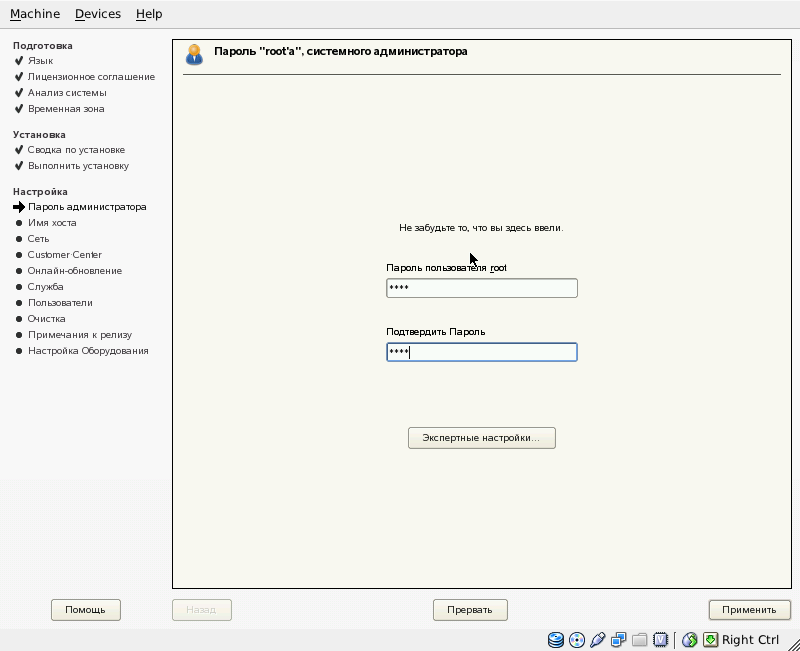
\includegraphics[width=1\linewidth]{oes/rootpasswd.png}}
\caption{Пароль системного администратора}
\label{fig6}
\end{figure}
\clearpage

Следующий этап это указание имени узла (в нашем случае oes2 - по названию операционной системы) и домена DNS (вариации на тему <имя компании>.ru).
\begin{figure}[H]
\center{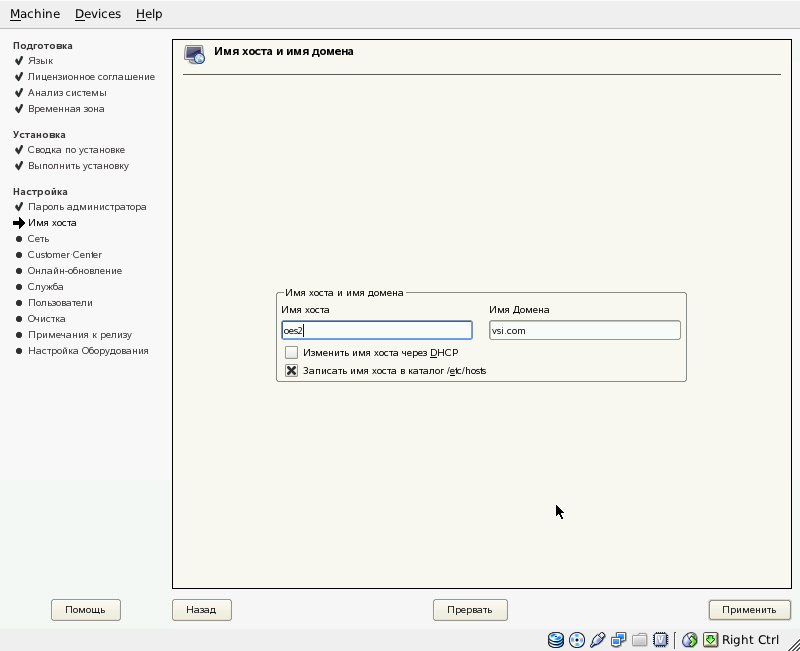
\includegraphics[width=1\linewidth]{oes/7.png}}
\caption{Имя хоста и имя домена}
\label{fig7}
\end{figure}
\clearpage

В разделе <<Настройка сети>> необходимо задать ip адрес сервера. По умолчанию сетевые адаптеры не настроены, либо настроены на использование DHCP, что совершенно не годится в случае с сервером. Для этого нажимаем <<Изменить>> и выбираем <<Сетевые интерфейсы>>.
\begin{figure}[H]
\center{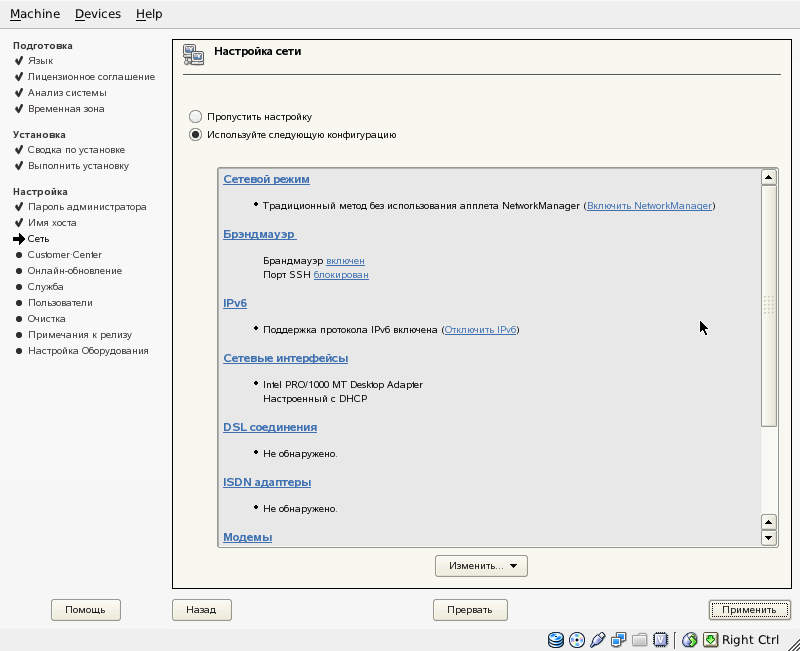
\includegraphics[width=1\linewidth]{oes/networkall.png}}
\caption{Настройка сети}
\label{figNetworkall}
\end{figure}
\clearpage

Сетевую карту необходимо настроить на статическое получение адреса — выбрать <<Установка статического адреса>> и задать все необходимые параметры: IP-адрес и маску подсети.
\begin{figure}[H]
\center{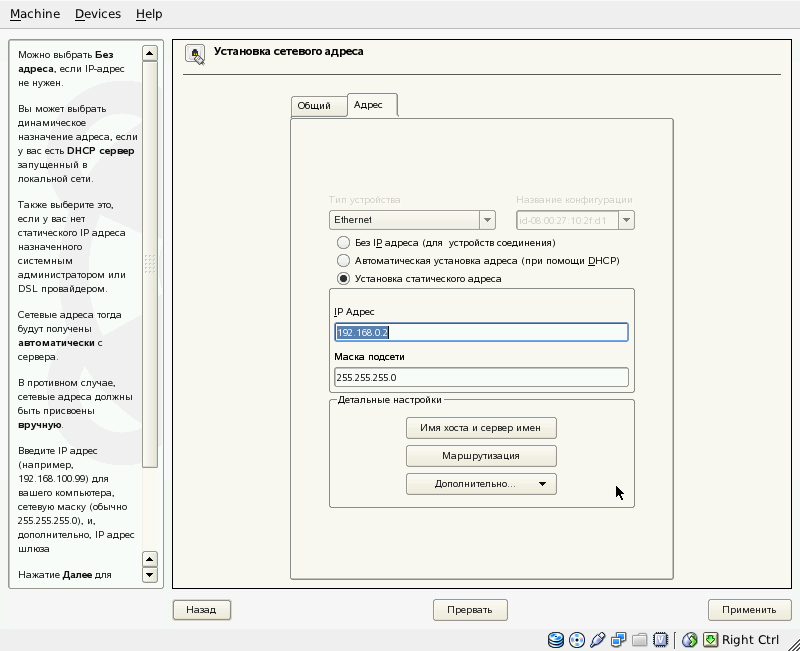
\includegraphics[width=1\linewidth]{oes/8.png}}
\caption{Настройка сетевого адреса}
\label{fig8}
\end{figure}
\clearpage

Следующим шагом будет настройка DNS. Жмём <<Имя хоста и сервер имён>> и прописываем наш сервер в <<Сервер имён 1>>. Завершаем настройку кнопкой <<Применить>>.
\begin{figure}[H]
\center{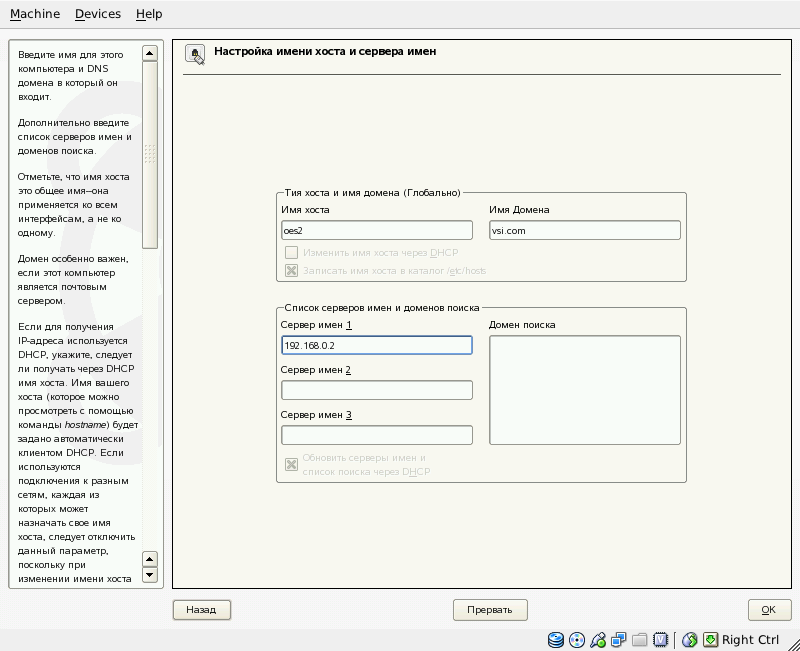
\includegraphics[width=1\linewidth]{oes/9.png}}
\caption{Настройка DNS}
\label{fig9}
\end{figure}
\clearpage

Теперь, когда сеть настроена, можно попробовать подключиться к сети Интернет и проверить последние обновления с сайта novell.com.
\begin{figure}[H]
\center{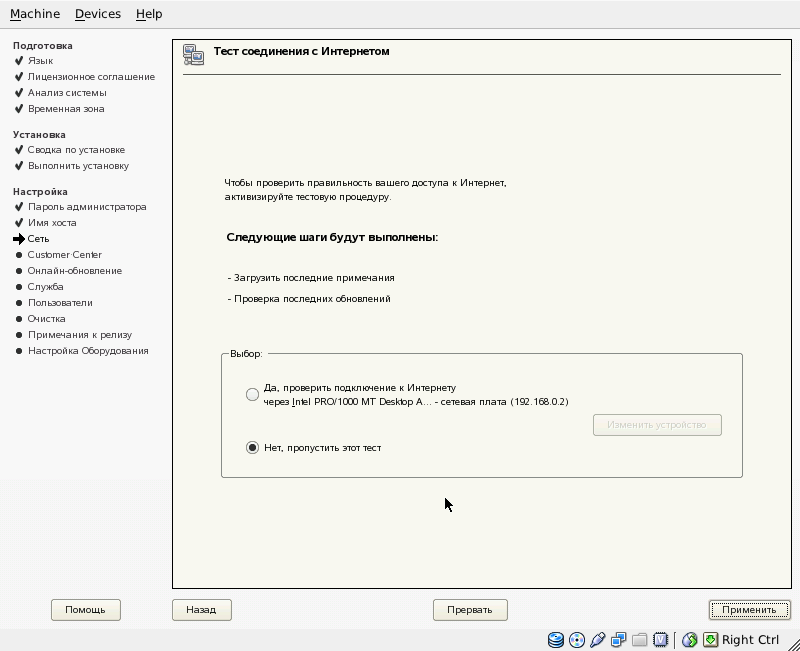
\includegraphics[width=1\linewidth]{oes/10.png}}
\caption{Тест соединения с Интернетом}
\label{fig10}
\end{figure}
Если на текущем этапе нет желания или возможности проверить подключение к сети Интернет, то выбираем вариант <<Нет, пропустить этот тест>>.
\clearpage

Ещё один тонкий момент, требующий внимания — настройка сертификата сервера. Как видно исходное значения поля <<Страна>> выставлено равным <<RU.KOI8-R>>, что не совсем правильно. 
\begin{figure}[H]
\center{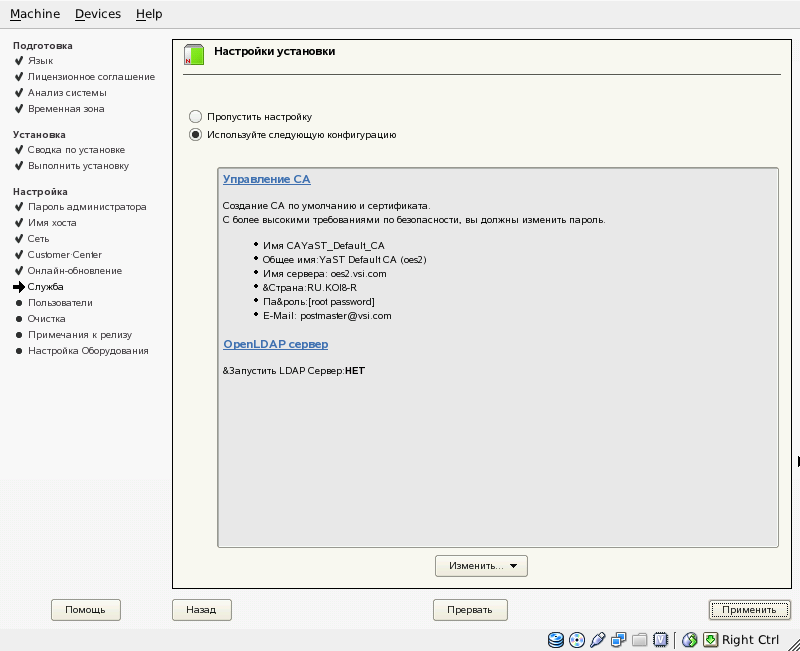
\includegraphics[width=1\linewidth]{oes/sertificate.png}}
\caption{CA сертификат}
\label{sertificate}
\end{figure}
Чтобы изменить параметры сертификата жмём линк <<Управление СА>>. 
\clearpage

В открывшемся окне находим кнопку <<Редактировать Установки по Умолчанию>> и меняем поле страна на Россия.
\begin{figure}[H]
\center{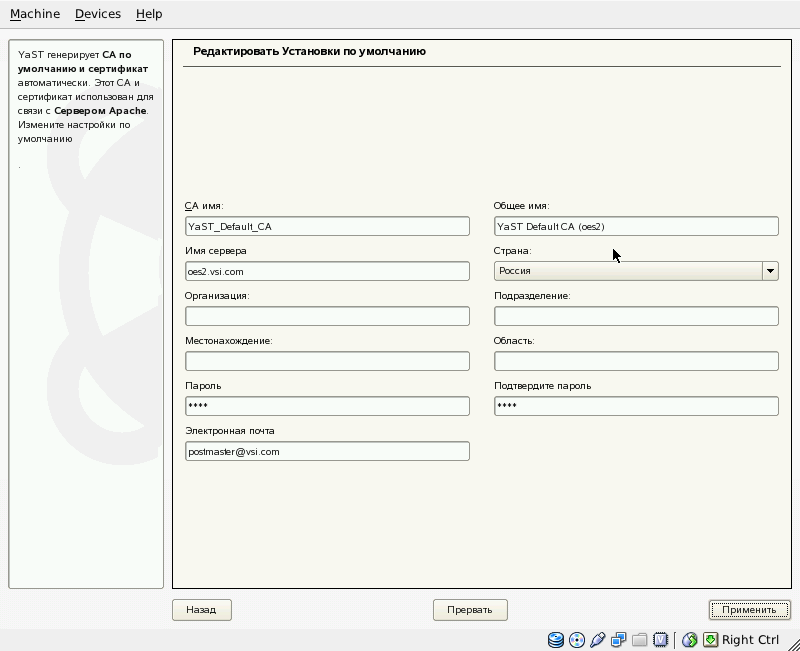
\includegraphics[width=1\linewidth]{oes/11.png}}
\caption{Редактирование CA сертификата}
\label{fig11}
\end{figure}
\clearpage

Следующий этап --- это создание локальных пользователей.
\begin{figure}[H]
\center{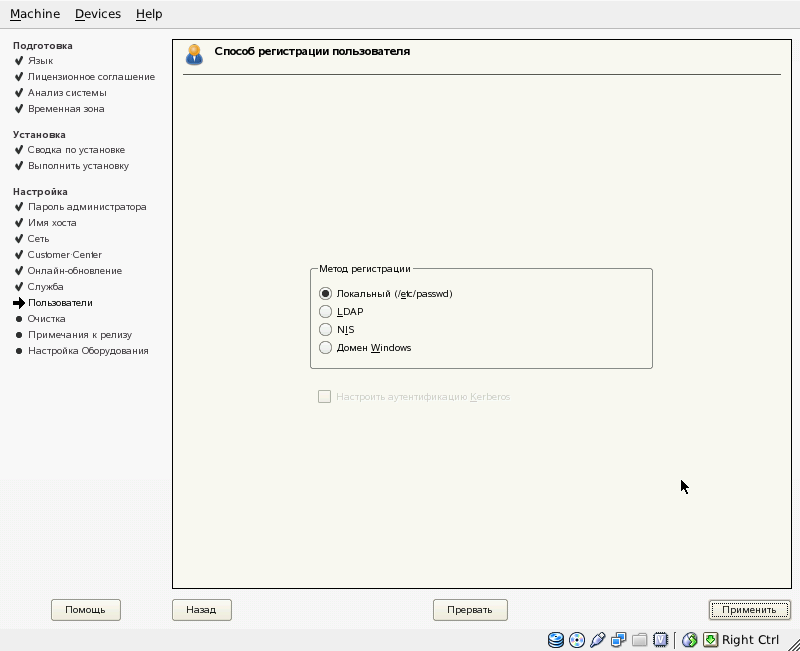
\includegraphics[width=1\linewidth]{oes/12.png}}
\caption{Способ регистрации пользователей}
\label{fig12}
\end{figure}
Выбираем метод регистрации <<Локальный (/etc/passwd)>>.
\clearpage

Произвольно задаём имя пользователя и пароль.
\begin{figure}[H]
\center{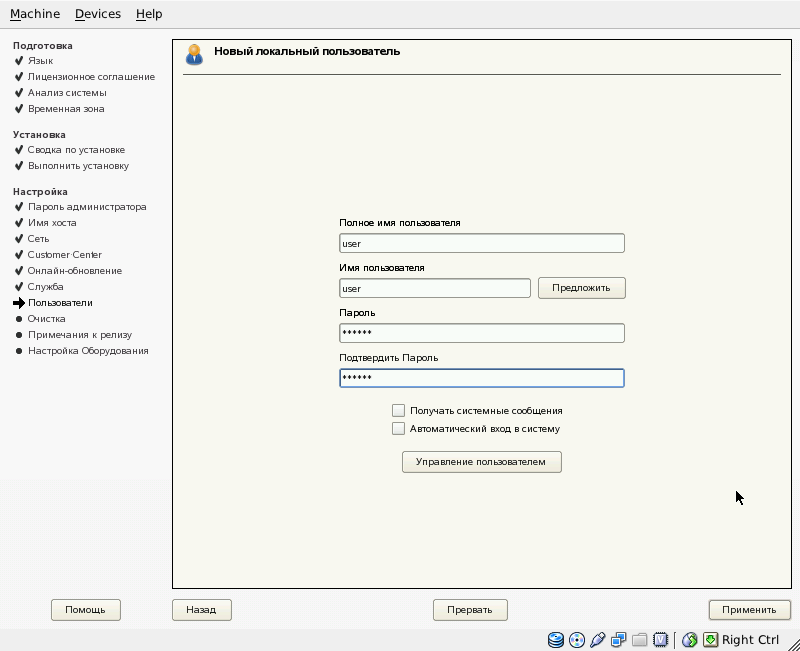
\includegraphics[width=1\linewidth]{oes/13.png}}
\caption{Создание локального пользователя}
\label{fig13}
\end{figure}
Жмём кнопку <<Применить>>, переходим к окну примечаний к выпуску и вновь жмём кнопку <<Применить>>.
\clearpage

Окно настройки оборудования показывает текущие настройки видеокарты, принтеров и звука. Оставляем всё без изменений.
\begin{figure}[H]
\center{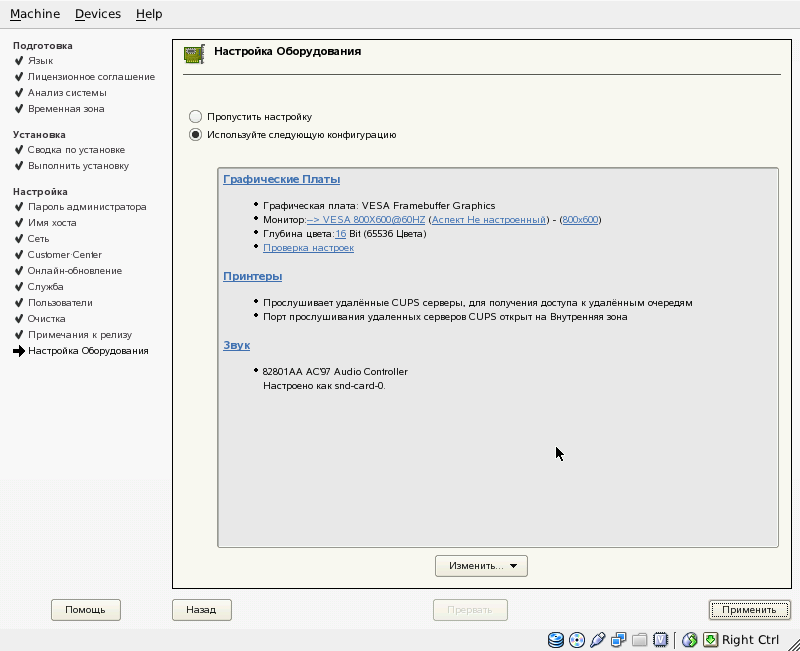
\includegraphics[width=1\linewidth]{oes/14.png}}
\caption{Настройка оборудования}
\label{fig14}
\end{figure}
\clearpage

Установка завершена, о чём нам и сообщает открывшееся окно. (рис.~\ref{fig15})
\begin{figure}[H]
\center{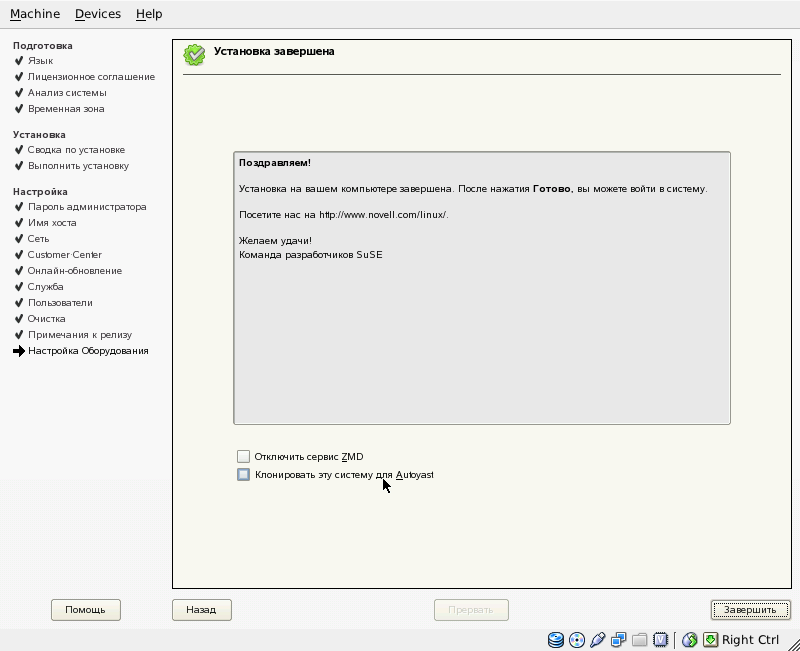
\includegraphics[width=1\linewidth]{oes/15.png}}
\caption{Завершение установки}
\label{fig15}
\end{figure}
Если мы хотим сохранить настройки для будущего клонирования операционной
системы, то ставим крестик в поле <<Клонировать эту систему для Autoyast>>. Жмём кнопку <<Завершить>>.
\clearpage

Теперь мы можем зайти на сервер локально и закончить настройку сервера.
\begin{figure}[H]
\center{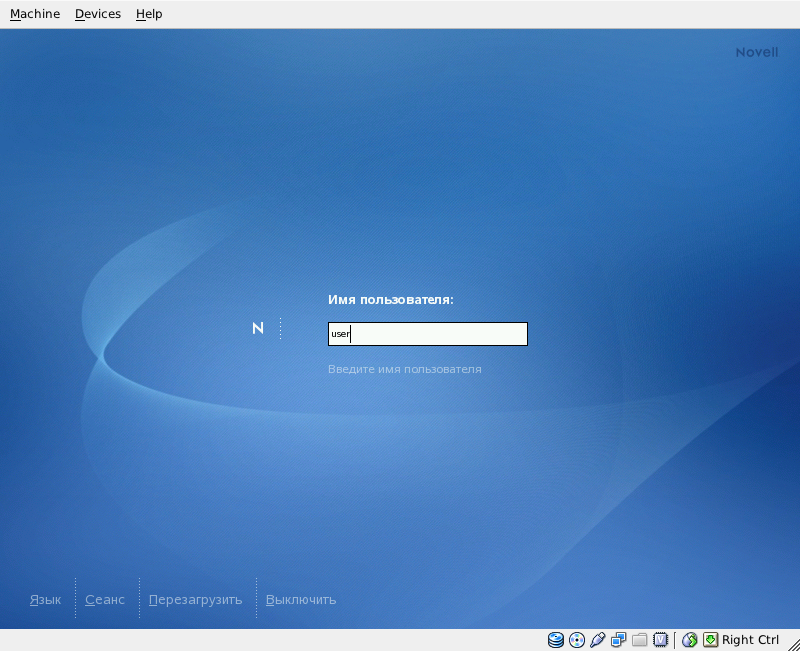
\includegraphics[width=1\linewidth]{oes/16.png}}
\caption{Вход в систему}
\label{fig16}
\end{figure}
\clearpage

\section{Настройка}
Open Enterprise Server основывается на linux дистрибутиве openSUSE\footnote{http://www.opensuse.org/ru/}, поэтому по вопросам использования или настройки можно воспользоваться любыми справочными материалами, посвящёнными этому дистрибутиву. Здесь мы коснёмся лишь настройке сервисов, относящихся к диску OES2.\par 
Все настройки ОС openSUSE пройзводятся с помощью менеджера YaST\footnote{http://ru.opensuse.org/YaST}.
\begin{figure}[H]
\center{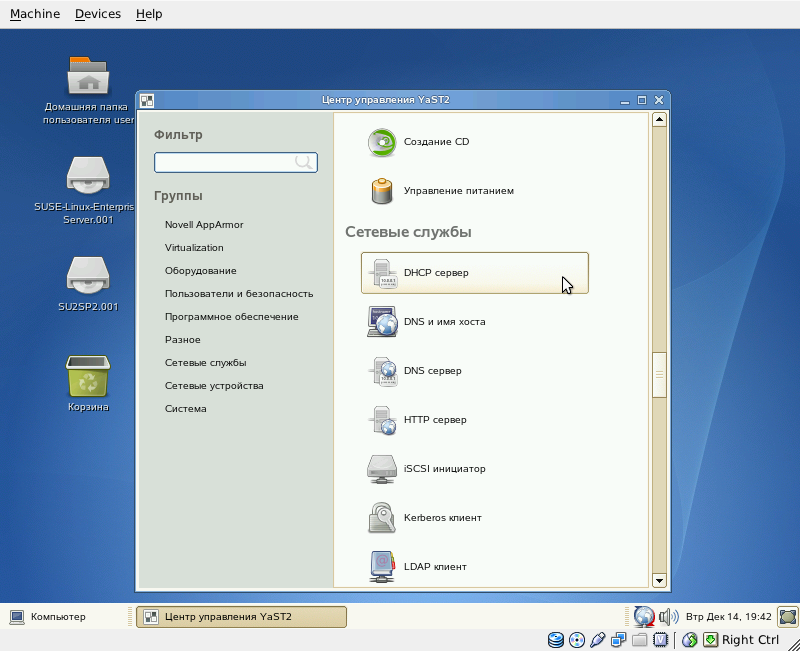
\includegraphics[width=1\linewidth]{oes/yast.png}}
\caption{YaST}
\label{yast}
\end{figure}
\clearpage

\subsection{DHCP}
Настройка DHCP здесь ничем принципиально не отличается от настройки в Windows системах. Выбирается сетевой интерфейс, на котором будут раздаваться IP адреса, также назначаются сервера имён и диапазон IP адресов. Последний шагом станет выбор, будет ли сервер стартовать при загрузке операционной системы или его следует запускать вручную.
\begin{figure}[H]
\center{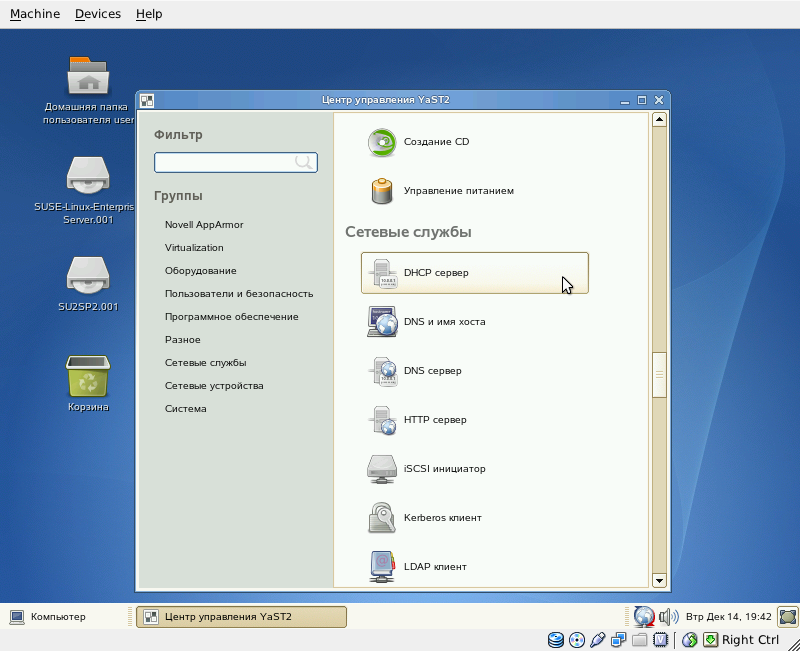
\includegraphics[width=1\linewidth]{oes/dhcp.png}}
\caption{Настройка DHCP}
\label{dhcp}
\end{figure}
В процессе настройки у системы может возникнуть желание доустановить недостающие компоненты. Для этого необходимо вставить соответствующий диск с ПО. Базовые пакеты находятся на дисках SLES, в то время как всё проприетарное программное обеспечение лежит на диске OES2.
\clearpage

\subsection{eDirectory}
Для настройки eDirectory\footnote{http://www.novell.com/russia/products/edirectory/} нам потребуется диск OES2. Заходим в YaST и находим пункт <<Дополнительный продукт>>. 
\begin{figure}[H]
\center{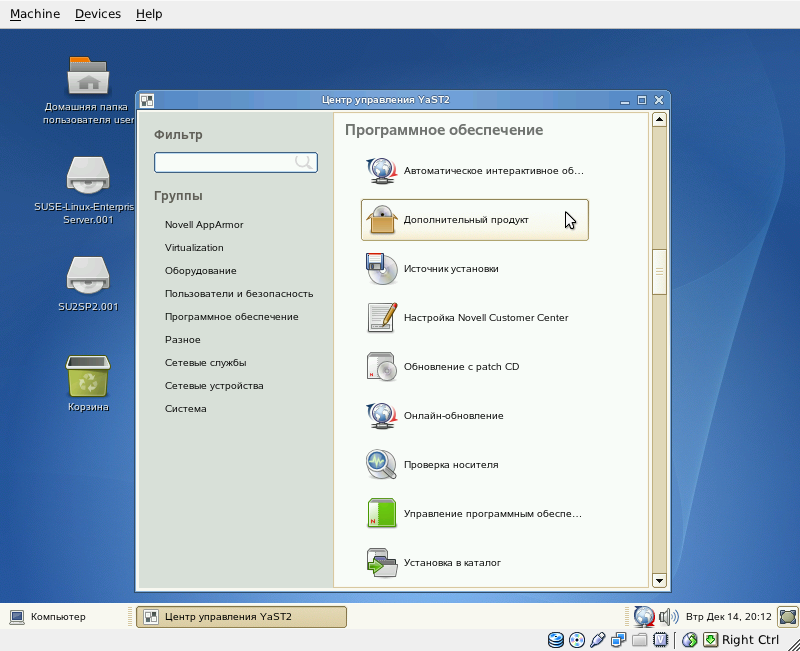
\includegraphics[width=1\linewidth]{oes/edir1.png}}
\caption{Установка дополнительного продукта}
\end{figure}
Если вдальнейшем понадобится какой-то компонент, это легко можно сделать через соответственную оснастку YaST.
\clearpage

В окне выбора носителя выбираем CD, нажимаем применить. В появившемся окне <<Вставьте CD с дополнительным продуктом>> нажимаем <<Извлечь>>, чтобы размонтировать и извлечь диск SLES. Вставляем диск с OES2 и нажимаем <<Продолжить>>.
\begin{figure}[H]
\center{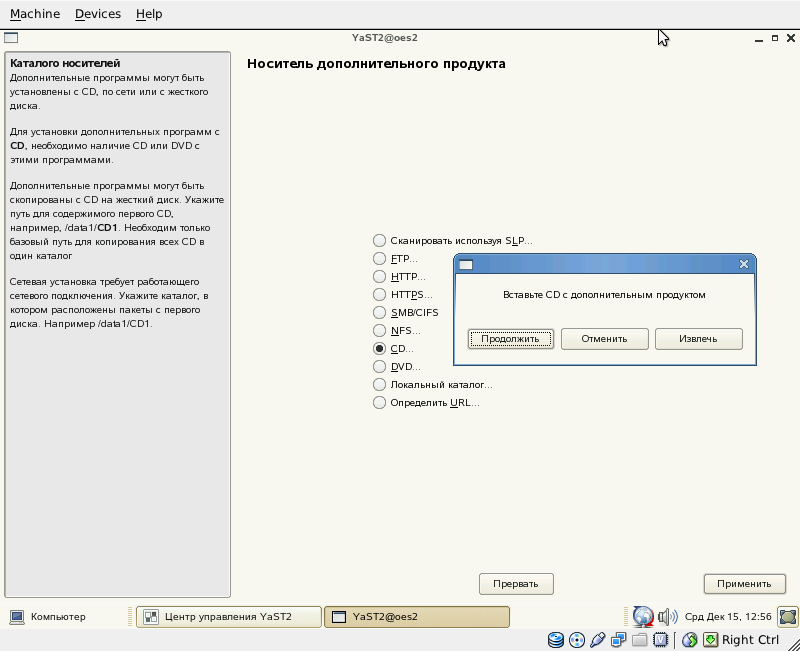
\includegraphics[width=1\linewidth]{oes/edir3.png}}
\caption{Выбор носителя}
\end{figure}
\clearpage

В новом окне всё доступное ПО разбито по группам. Нас интересует группа <<Сервисы OES>>. Выбираем <<Доменные службы Novell для Windows>> - ставим галочку напротив строчки. Все зависимости будут проставлены автоматически. Также выбираем <<Novell iManager>>\footnote{http://www.novell.com/ru-ru/documentation/imanager27/} - средство удалённого администрирования сервера.
\begin{figure}[H]
\center{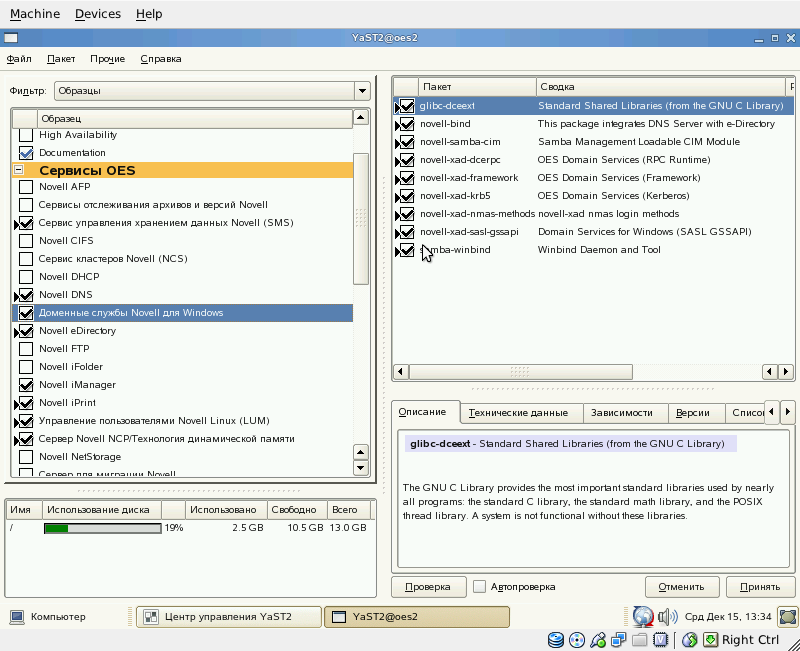
\includegraphics[width=1\linewidth]{oes/edir5.png}}
\caption{Выбор компонентов}
\end{figure}
Нажимаем принять, и приступаем к установке.
\clearpage

Всякий раз когда нас попросят вставить следующий диск с ПО, нужно не забывать нажимать кнопку <<Извлечь>>, чтобы диск размонтировался.
\begin{figure}[H]
\center{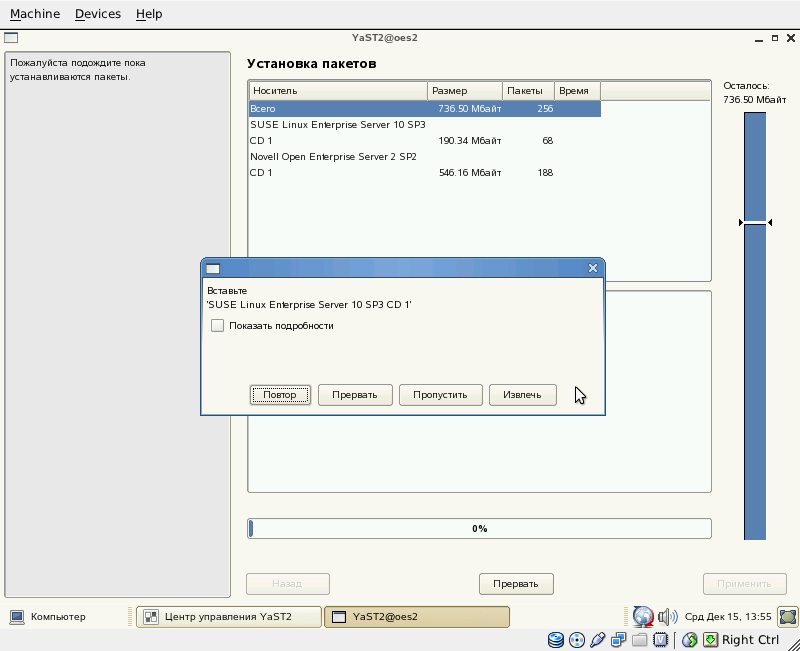
\includegraphics[width=1\linewidth]{oes/edir6.png}}
\caption{Новый носитель}
\end{figure}
\clearpage

После установки всех пакетов начинается настройка самой важной части сети --- сетевого каталога eDirectory.
\begin{figure}[H]
\center{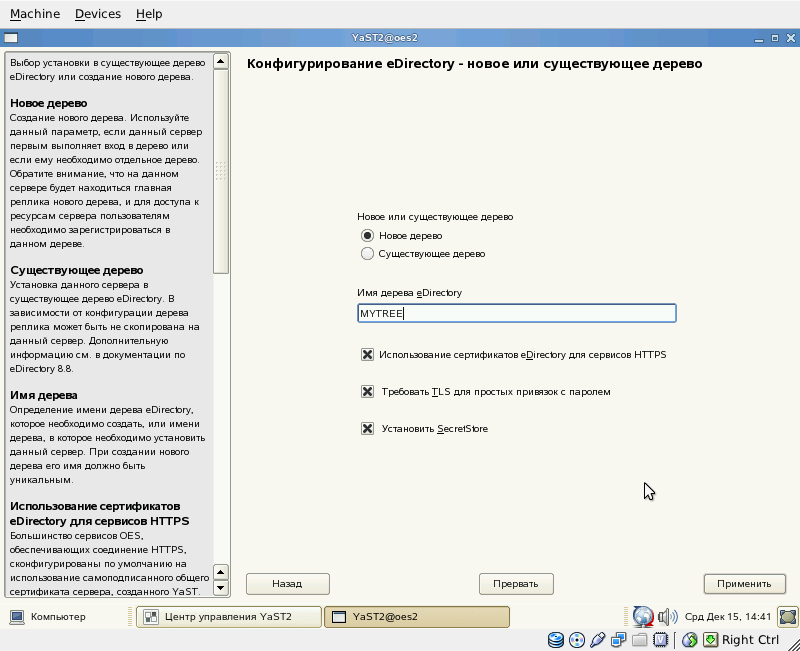
\includegraphics[width=1\linewidth]{oes/edir7.png}}
\caption{Новое или существующее дерево}
\end{figure}
Мы выберем <<Новое дерево>> и зададим имя <<MYTREE>>. Крестик в поле <<Использование сертификатов eDirectory для сервисов HTTPS>> означает что сертификат будет заменён на на тот, который мы создавали при установке.
\clearpage

Второй этап настройки eDirectory --- создание учётной записи администратора сетевого каталога. Это не то же самое, что и root. Права у них сильно различаются. root ничего не может сделать с сетевым каталогом, кроме как полностью удалить его со своего сервера (но не во всей сети). Администратор каталога сильно ограничен в правах на локальную файловую систему сервера, но может стереть сетевой каталог со всей сети сразу.
\begin{figure}[H]
\center{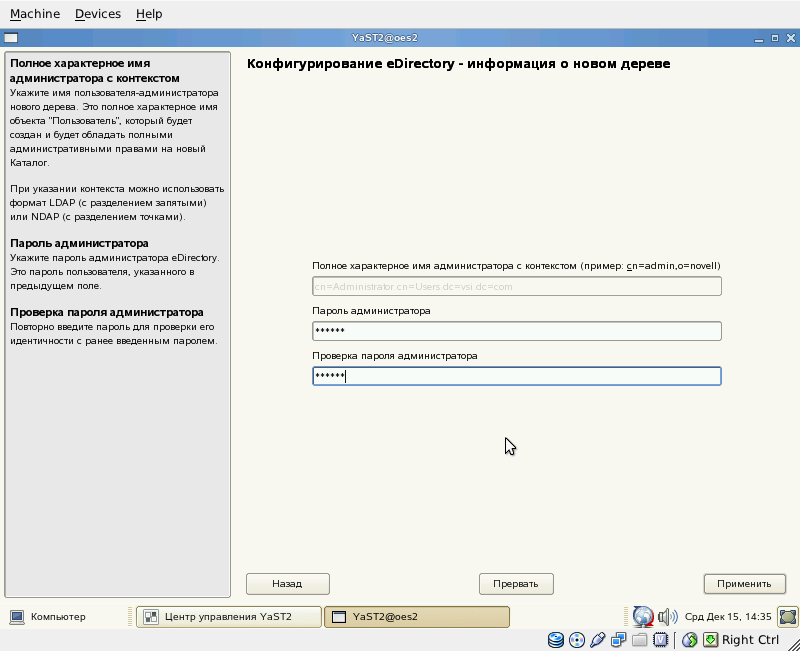
\includegraphics[width=1\linewidth]{oes/edir8.png}}
\caption{Пароль администратора домена}
\end{figure}
Само имя администратора уже задано и не изменяется, необходимо лишь вписать пароль.
\clearpage

Настройка, не требующая изменений в обычной жизни: местонахождение сервера и базы данных каталога, порты LDAP и веб-мониторинга.
\begin{figure}[H]
\center{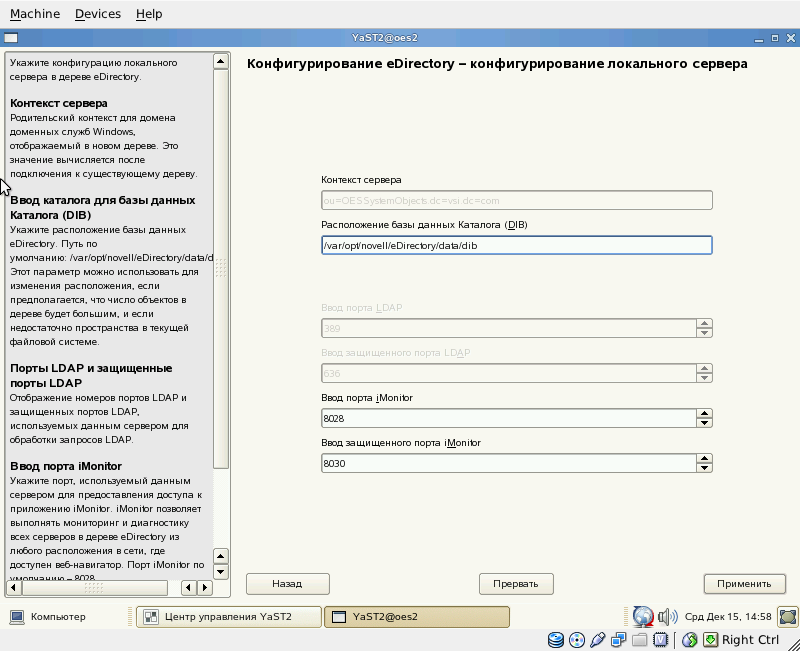
\includegraphics[width=1\linewidth]{oes/edir9.png}}
\caption{Конфигурирование локального сервера}
\end{figure}
Сразу жмём <<Применить>>.
\clearpage

На следующем экране предлагается настройка времени и протокола обнаружения служб.
\begin{figure}[H]
\center{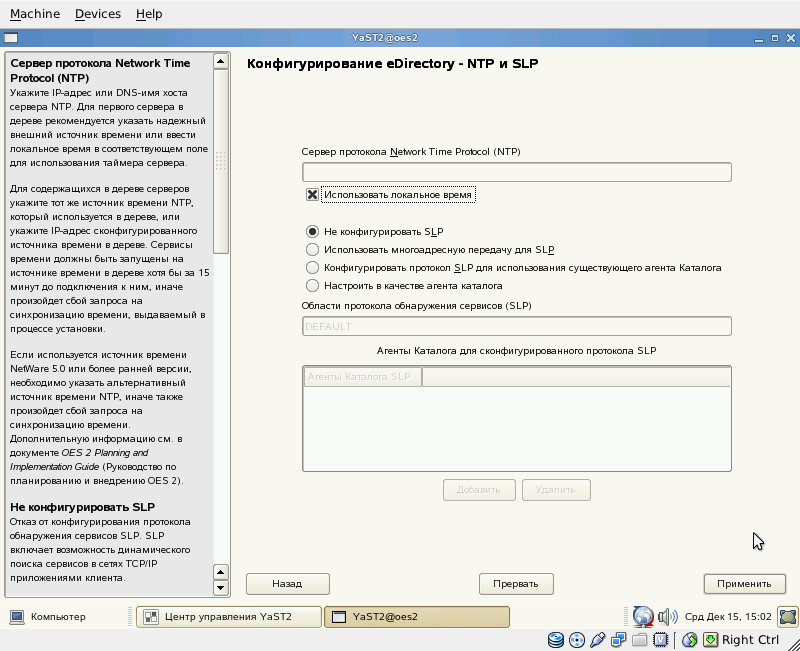
\includegraphics[width=1\linewidth]{oes/edir10.png}}
\caption{NTP и SLP}
\end{figure}
Аккуратная настройка времени между серверами обязательна! Для одного сервера можно использовать локальное время. Когда же соберётесь ставить второй и все последующие сервера, обязательно заводите их на единый источник времени и не допускайте рассинхронизации между серверами больше чем на несколько минут.\par
Service Location Protocol (SLP) --- это специальный протокол, разработанный для обнаружения различных сервисов в сети. На текущем этапе мы его не настраиваем.
\clearpage

Этап настройки NMAS пропускаем без изменений, т.к. исходные значения подходят практически для каждой установки.
\begin{figure}[H]
\center{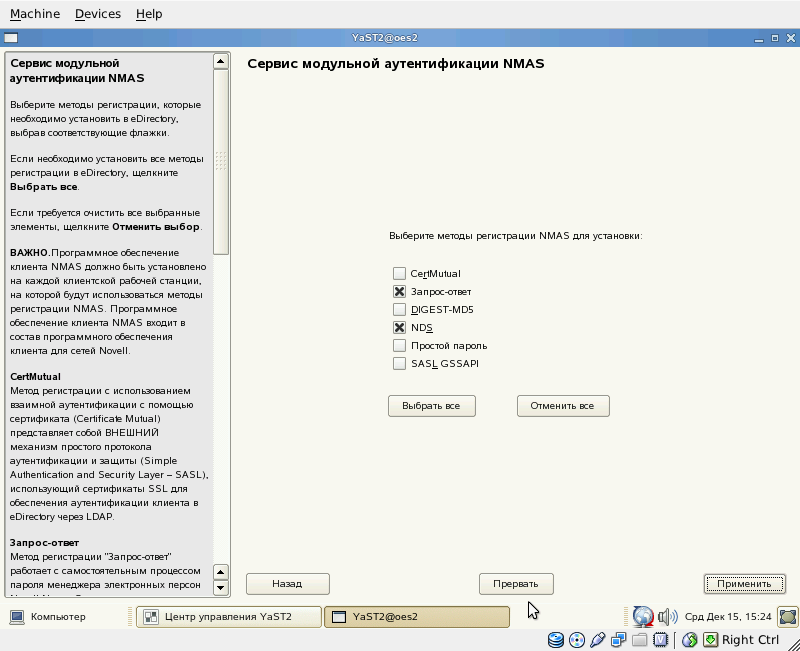
\includegraphics[width=1\linewidth]{oes/edir11.png}}
\caption{Методы регистрации NMAS}
\end{figure}
\clearpage

Теперь пришла очередь настройки домена Windows. Так как в сети нет ни одного сервера Windows с доменной службой, то доступен единственный вариант --- <<Новые доменные службы для леса Windows>>. Имена DNS и NetBIOS для нового домена взяты из предыдущих настроек. 
\begin{figure}[H]
\center{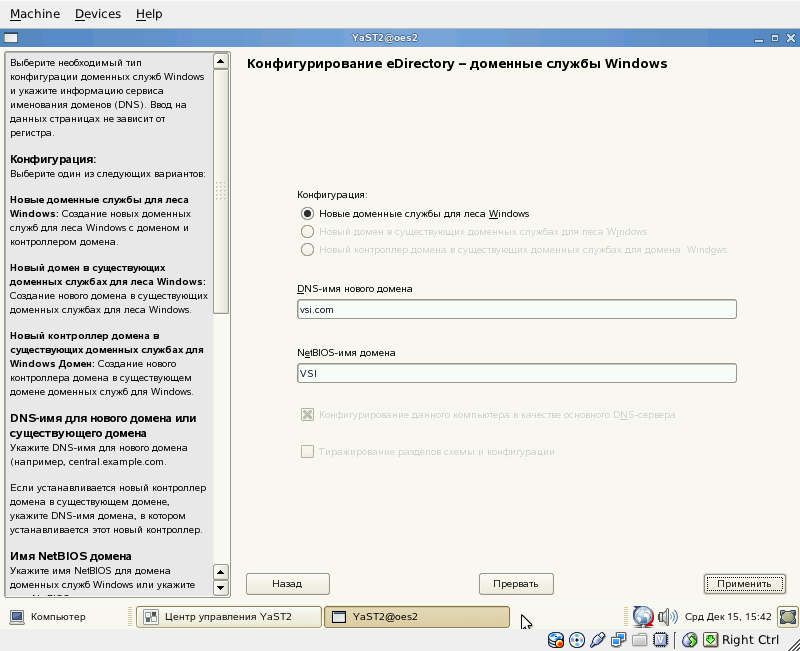
\includegraphics[width=1\linewidth]{oes/edir12.png}}
\caption{Доменные службы Windows}
\end{figure}
\clearpage

Теперь следует настроить службу DNS. Для продолжения нужно указать имя нового пользователя, у которого будут права на управление eDirectory (например cn=dnsadmin,dc=vsi,dc=com) и его пароль с подтверждением.
\begin{figure}[H]
\center{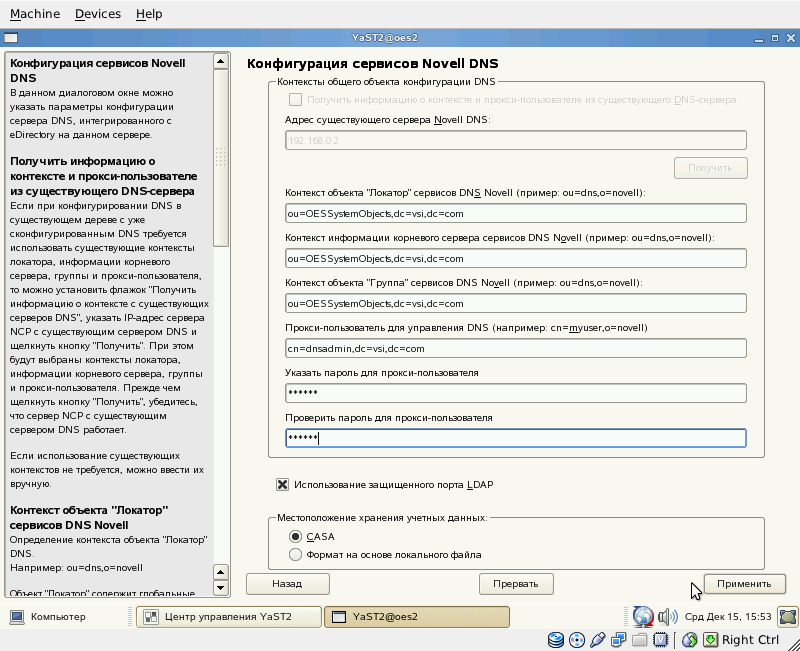
\includegraphics[width=1\linewidth]{oes/edir13.png}}
\caption{Конфигурация DNS}
\end{figure}
\clearpage

Вот и добрались до настройки сервисов Novell. К счастью здесь ничего не нужно настраивать вручную, всё настроено автоматически на использование текущего дерева каталога.
\begin{figure}[H]
\center{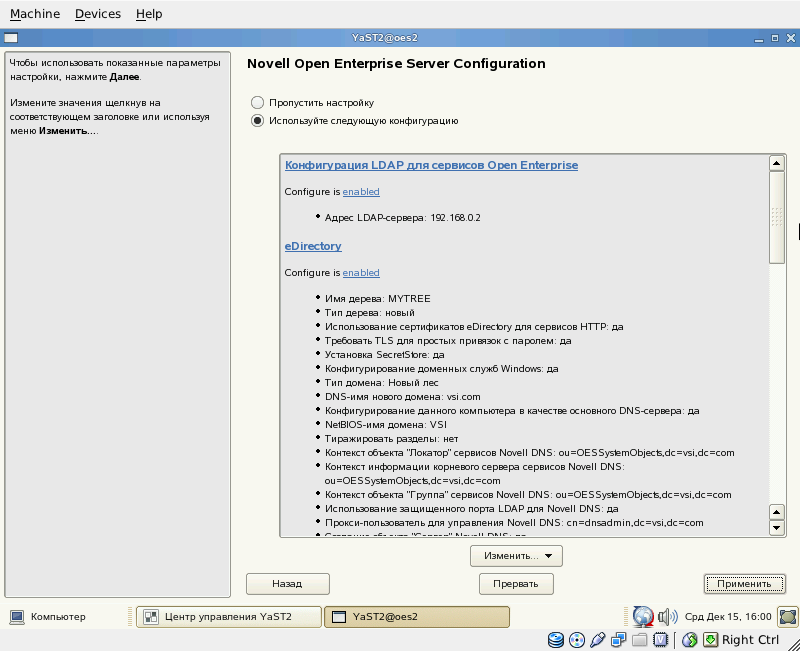
\includegraphics[width=1\linewidth]{oes/edir14.png}}
\caption{Конфигурация сервисов Novell}
\end{figure}
Завершаем настройку, нажав кнопку <<Применить>>.

\clearpage
\section{Настройка клиента}
Установка Novell Client\footnote{http://www.novell.com/products/clients/}